%%%%%%%%%%%%%%%%%%%%%%%%%%%%%%%%%%%%%%%%%
% Masters/Doctoral Thesis 
% LaTeX Template
% Version 2.2 (21/11/15)
%
% This template has been downloaded from:
% http://www.LaTeXTemplates.com
%
% Version 2.x major modifications by:
% Vel (vel@latextemplates.com)
%
% This template is based on a template by:
% Steve Gunn (http://users.ecs.soton.ac.uk/srg/softwaretools/document/templates/)
% Sunil Patel (http://www.sunilpatel.co.uk/thesis-template/)
%
% Template license:
% CC BY-NC-SA 3.0 (http://creativecommons.org/licenses/by-nc-sa/3.0/)
%
%%%%%%%%%%%%%%%%%%%%%%%%%%%%%%%%%%%%%%%%%

%----------------------------------------------------------------------------------------
%	PACKAGES AND OTHER DOCUMENT CONFIGURATIONS
%----------------------------------------------------------------------------------------

\documentclass[
11pt, % The default document font size, options: 10pt, 11pt, 12pt
oneside, % Two side (alternating margins) for binding by default, uncomment to switch to one side
english, % ngerman for German
singlespacing, % Single line spacing, alternatives: onehalfspacing or doublespacing
%draft, % Uncomment to enable draft mode (no pictures, no links, overfull hboxes indicated)
%nolistspacing, % If the document is onehalfspacing or doublespacing, uncomment this to set spacing in lists to single
%liststotoc, % Uncomment to add the list of figures/tables/etc to the table of contents
%toctotoc, % Uncomment to add the main table of contents to the table of contents
%parskip, % Uncomment to add space between paragraphs
%nohyperref, % Uncomment to not load the hyperref package
headsepline, % Uncomment to get a line under the header
]{MastersDoctoralThesis} % The class file specifying the document structure

\usepackage[UTF8, heading = false, scheme = plain]{ctex}

\usepackage[utf8]{inputenc} % Required for inputting international characters
\usepackage[T1]{fontenc} % Output font encoding for international characters
\usepackage{palatino} % Use the Palatino font by default


\usepackage[backend=bibtex,style=authoryear,natbib=true]{biblatex} % User the bibtex backend with the authoryear citation style (which resembles APA)

\addbibresource{example.bib} % The filename of the bibliography

\usepackage[autostyle=true]{csquotes} % Required to generate language-dependent quotes in the bibliography

\usepackage{float}
\usepackage{multirow}
\usepackage{longtable}
\usepackage{enumerate}

\usepackage{indentfirst}
\setlength{\parindent}{2em}
\setlength{\parskip}{7pt}
\linespread{1.2}

%----------------------------------------------------------------------------------------
%	MARGIN SETTINGS
%----------------------------------------------------------------------------------------

\geometry{
	paper=a4paper, % Change to letterpaper for US letter
	inner=3.5cm, % Inner margin
	outer=3.5cm, % Outer margin
	%bindingoffset=2cm, % Binding offset
	top=2cm, % Top margin
	bottom=2cm, % Bottom margin
	%showframe,% show how the type block is set on the page
}

%----------------------------------------------------------------------------------------
%	THESIS INFORMATION
%----------------------------------------------------------------------------------------

\thesistitle{数据库课程项目报告} % Your thesis title, this is used in the title and abstract, print it elsewhere with \ttitle
\supervisor{冯建华、张勇} % Your supervisor's name, this is used in the title page, print it elsewhere with \supname
\examiner{} % Your examiner's name, this is not currently used anywhere in the template, print it elsewhere with \examname
\degree{} % Your degree name, this is used in the title page and abstract, print it elsewhere with \degreename
\author{桥本优、钱雨杰、董胤蓬} % Your name, this is used in the title page and abstract, print it elsewhere with \authorname
\addresses{} % Your address, this is not currently used anywhere in the template, print it elsewhere with \addressname

\subject{Computer Sciences and Technology} % Your subject area, this is not currently used anywhere in the template, print it elsewhere with \subjectname
\keywords{} % Keywords for your thesis, this is not currently used anywhere in the template, print it elsewhere with \keywordnames
\university{\href{http://www.tsinghua.edu.cn}{清华大学}} % Your university's name and URL, this is used in the title page and abstract, print it elsewhere with \univname
\department{\href{http://department.university.com}{计算机科学与技术系}} % Your department's name and URL, this is used in the title page and abstract, print it elsewhere with \deptname
\group{\href{http://researchgroup.university.com}{Research Group Name}} % Your research group's name and URL, this is used in the title page, print it elsewhere with \groupname
\faculty{\href{http://faculty.university.com}{Faculty Name}} % Your faculty's name and URL, this is used in the title page and abstract, print it elsewhere with \facname

\hypersetup{pdftitle=\ttitle} % Set the PDF's title to your title
\hypersetup{pdfauthor=\authorname} % Set the PDF's author to your name
\hypersetup{pdfkeywords=\keywordnames} % Set the PDF's keywords to your keywords

\begin{document}

\frontmatter % Use roman page numbering style (i, ii, iii, iv...) for the pre-content pages

\pagestyle{plain} % Default to the plain heading style until the thesis style is called for the body content

%----------------------------------------------------------------------------------------
%	TITLE PAGE
%----------------------------------------------------------------------------------------

\begin{titlepage}
\begin{center}

\includegraphics[width=0.3\textwidth]{Figures/thu.png}\\[1cm]
\textsc{\LARGE \univname}\\[0.8cm] % University name
\textsc{\LARGE 数据库系统概论}\\[0.5 cm] % Thesis type

\HRule \\[0.8cm] % Horizontal line
{\huge \bfseries \ttitle}\\[0.4cm] % Thesis title
%\large \textit{课程项目报告}\\[0.3cm] % University requirement text
\HRule \\[1.5cm] % Horizontal line
 
\begin{minipage}{0.4\textwidth}
\begin{flushleft} \large
\emph{作者:}\\[0.4cm] 
\authorname % Author name - remove the \href bracket to remove the link
\end{flushleft}
\end{minipage}
\begin{minipage}{0.4\textwidth}
\begin{flushright} \large
\emph{指导教师:} \\[0.4cm]
\supname % Supervisor name - remove the \href bracket to remove the link  
\end{flushright}
\end{minipage}\\[4cm]

%\textit{in the}\\[0.4cm]
\univname\\[0.1cm]\deptname\\[2cm] % Research group name and department name
 
{\large \today}\\[3cm] % Date
%\includegraphics{Logo} % University/department logo - uncomment to place it
 
\vfill
\end{center}
\end{titlepage}

%----------------------------------------------------------------------------------------
%	ABSTRACT PAGE
%----------------------------------------------------------------------------------------


%----------------------------------------------------------------------------------------
%	LIST OF CONTENTS/FIGURES/TABLES PAGES
%----------------------------------------------------------------------------------------

\tableofcontents % Prints the main table of contents

%\listoffigures % Prints the list of figures

%\listoftables % Prints the list of tables


%----------------------------------------------------------------------------------------
%	THESIS CONTENT - CHAPTERS
%----------------------------------------------------------------------------------------

\mainmatter % Begin numeric (1,2,3...) page numbering

\pagestyle{thesis} % Return the page headers back to the "thesis" style

% Include the chapters of the thesis as separate files from the Chapters folder
% Uncomment the lines as you write the chapters

% Chapter 1

\chapter{项目任务} % Main chapter title

\label{Chapter1} % For referencing the chapter elsewhere, use \ref{Chapter1} 

%----------------------------------------------------------------------------------------

% Define some commands to keep the formatting separated from the content 
\newcommand{\keyword}[1]{\textbf{#1}}
\newcommand{\tabhead}[1]{\textbf{#1}}
\newcommand{\code}[1]{\texttt{#1}}
\newcommand{\file}[1]{\texttt{\bfseries#1}}
\newcommand{\option}[1]{\texttt{\itshape#1}}

本项目是清华大学计算机科学与技术系开设的《数据库系统概论》课程项目。

项目的任务是实现一个单用户的关系数据库管理系统。该项目分为四个功能模块:
\begin{enumerate}[(1)]
\item 记录管理模块:该模块是DBMS的文件系统,管理存储数据库记录以及元数据的文件。该模块依赖于我们预先给定的一个页式文件I/O系统,在此基础上扩展而成。
\item 索引模块:为存储在文件中的记录建立B+树索引,加快查找速度。
\item 系统管理模块:实现基本的数据定义语言(DDL),实现解析器来解析命令行。
\item 查询解析模块:解析SQL语句,能将输入的SQL语句解析成关系代数表达式,并生成查询执行计划,访问文件系统执行查询,输出查询结果。
\end{enumerate}

在上述功能的基础上, 还可以对该系统进行个性化的功能扩展及性能优化,内容包括但不限于:
\begin{enumerate}[(1)] 
\item 查询优化:基于对查询计划代价的估计,为给定查询选择最有效的查询执行计划。
\item 支持属性域约束和外键约束。
\item 创建数据表时支持更多的数据类型。例如decimal, date等。
\item 支持三个或以上表的连接。
\item 支持更多SQL语句。例如聚集查询AVG,SUM,MIN,MAX,GROUP BY等。
\item 支持模糊查询。例如LIKE关键字以及“$\%$, *, ?”等通配符。
\item 提供类似MySQL front的图形化UI。
\end{enumerate}


%----------------------------------------------------------------------------------------


% Chapter Template

\chapter{系统结构设计} % Main chapter title

\label{Chapter2} % Change X to a consecutive number; for referencing this chapter elsewhere, use \ref{ChapterX}

%----------------------------------------------------------------------------------------
%	SECTION 1
%----------------------------------------------------------------------------------------

\section{系统架构}

 
% Chapter Template

\chapter{模块设计} % Main chapter title

\label{Chapter3} % Change X to a consecutive number; for referencing this chapter elsewhere, use \ref{ChapterX}

\section{记录管理模块}
记录管理模块主要负责在数据库中创建、打开、删除一个数据表,在表中插入、删除、更新一条记录,以及遍历表找到所有符合条件的记录。

我们在项目中把每张数据表存在独立的文件中。文件均由页式文件系统管理,每个数据表文件的第一页是表文件头页,记录整个数据表的一些信息;之后的页均为数据页,每个数据页的页头记录该页的一些信息。

具体地,表文件头页按以下格式组织:
\begin{figure}[H]
\centering
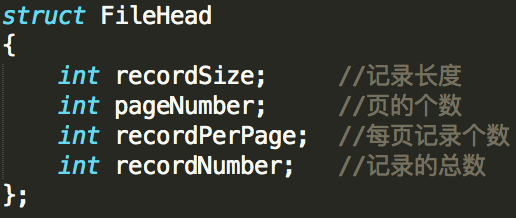
\includegraphics[width=3in]{Figures/FileHead.png}
\end{figure}
表文件头页中依次记4个整数,分别表示该表中记录长度、页的个数、每页的记录个数和表中记录总数。文件头页其余位置留空,可以用作其他扩展。

数据页每页8KB,前96 byte为页头,记录该页的一些信息,之后依次是固定长度的槽,每个槽可以放一条记录。数据页头按以下格式组织:
\begin{figure}[H]
\centering
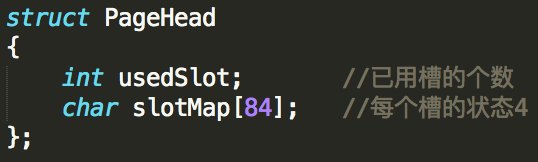
\includegraphics[width=3in]{Figures/PageHead.png}
\end{figure}
数据页头首先存放一个整数,记录本页已经放了几条记录。之后84 byte中每一个bit依次对应之后每个槽的状态,0表示为空,1表示已经有记录。

本模块的实现主要包括3个类,分别是RM\_Manager、RM\_FileHandle 以及 RM\_FileScan。在实现各个功能时,使用和维护之前所述的文件头、页头的信息。

\begin{figure}[H]
\centering
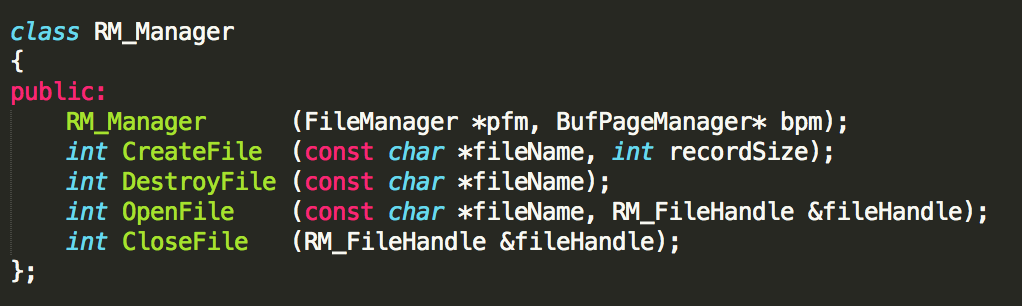
\includegraphics[width=5in]{Figures/RM_Manager.png}
\end{figure}

RM\_Manager提供的接口包括:(1)CreateFile:新建一个文件,生成表文件头页;(2)DestroyFile:删除一个文件;(3)OpenFile:打开一个文件,得到一个RM\_FileHandle,可以通过其进行对记录的操作;(4)CloseFile:关闭一个文件。

\begin{figure}[H]
\centering
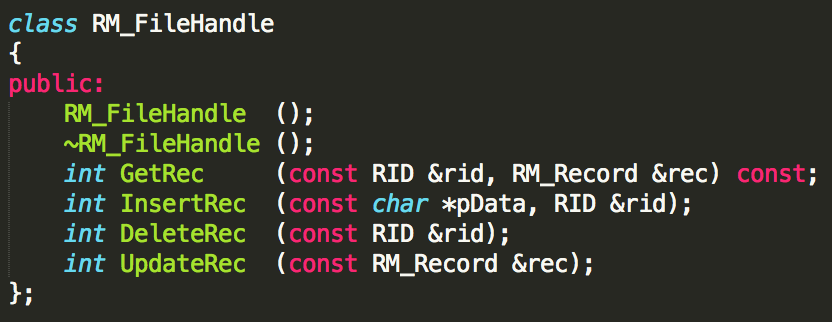
\includegraphics[width=4.5in]{Figures/RM_FileHandle.png}
\end{figure}

RM\_FileHandle提供的接口包括:(1)GetRec:根据RID获得记录内容;(2)InsertRec:插入一条记录,返回位置标识RID;(3)DeleteRec:根据RID删除一条记录;(4)UpdateRec:更新一个记录(知晓RID)。

\begin{figure}[H]
\centering
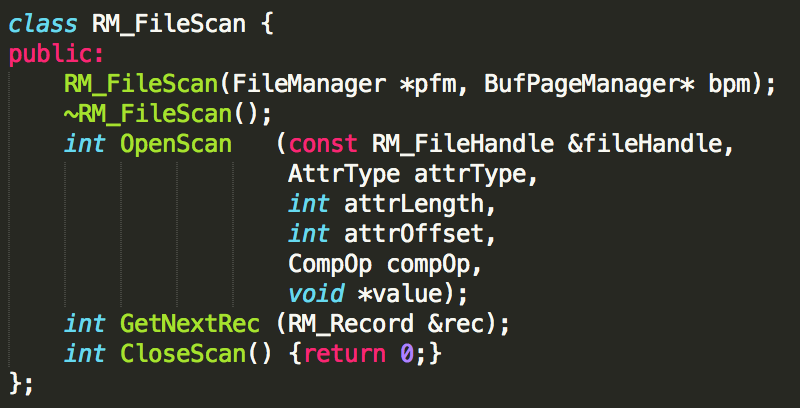
\includegraphics[width=4.2in]{Figures/RM_FileScan.png}
\end{figure}

RM\_FileScan提供的接口包括:(1)打开一个Scan,指定数据类型、长度、位置、约束条件;(2)获得一条符合条件的记录;(3)关闭一个Scan。

\section{系统管理模块}
系统管理模块中需要完成以下几个操作:(1)CREATE Database:新建一个数据库;(2)DROP Database:删除一个数据库;(3)USE Database:使用一个数据库;(4)CREATE TABLE tableName(attrName1 Type1, attrName2 Type2,…, attrNameN TypeN NOT NULL, PRIMARY KEY(attrName1):新建表,这里实现了Not NULL和Primary key两个关键字;(5)Show Database:显示这个数据库。

系统管理模块的类的定义如下:

\begin{figure}[H]
\centering
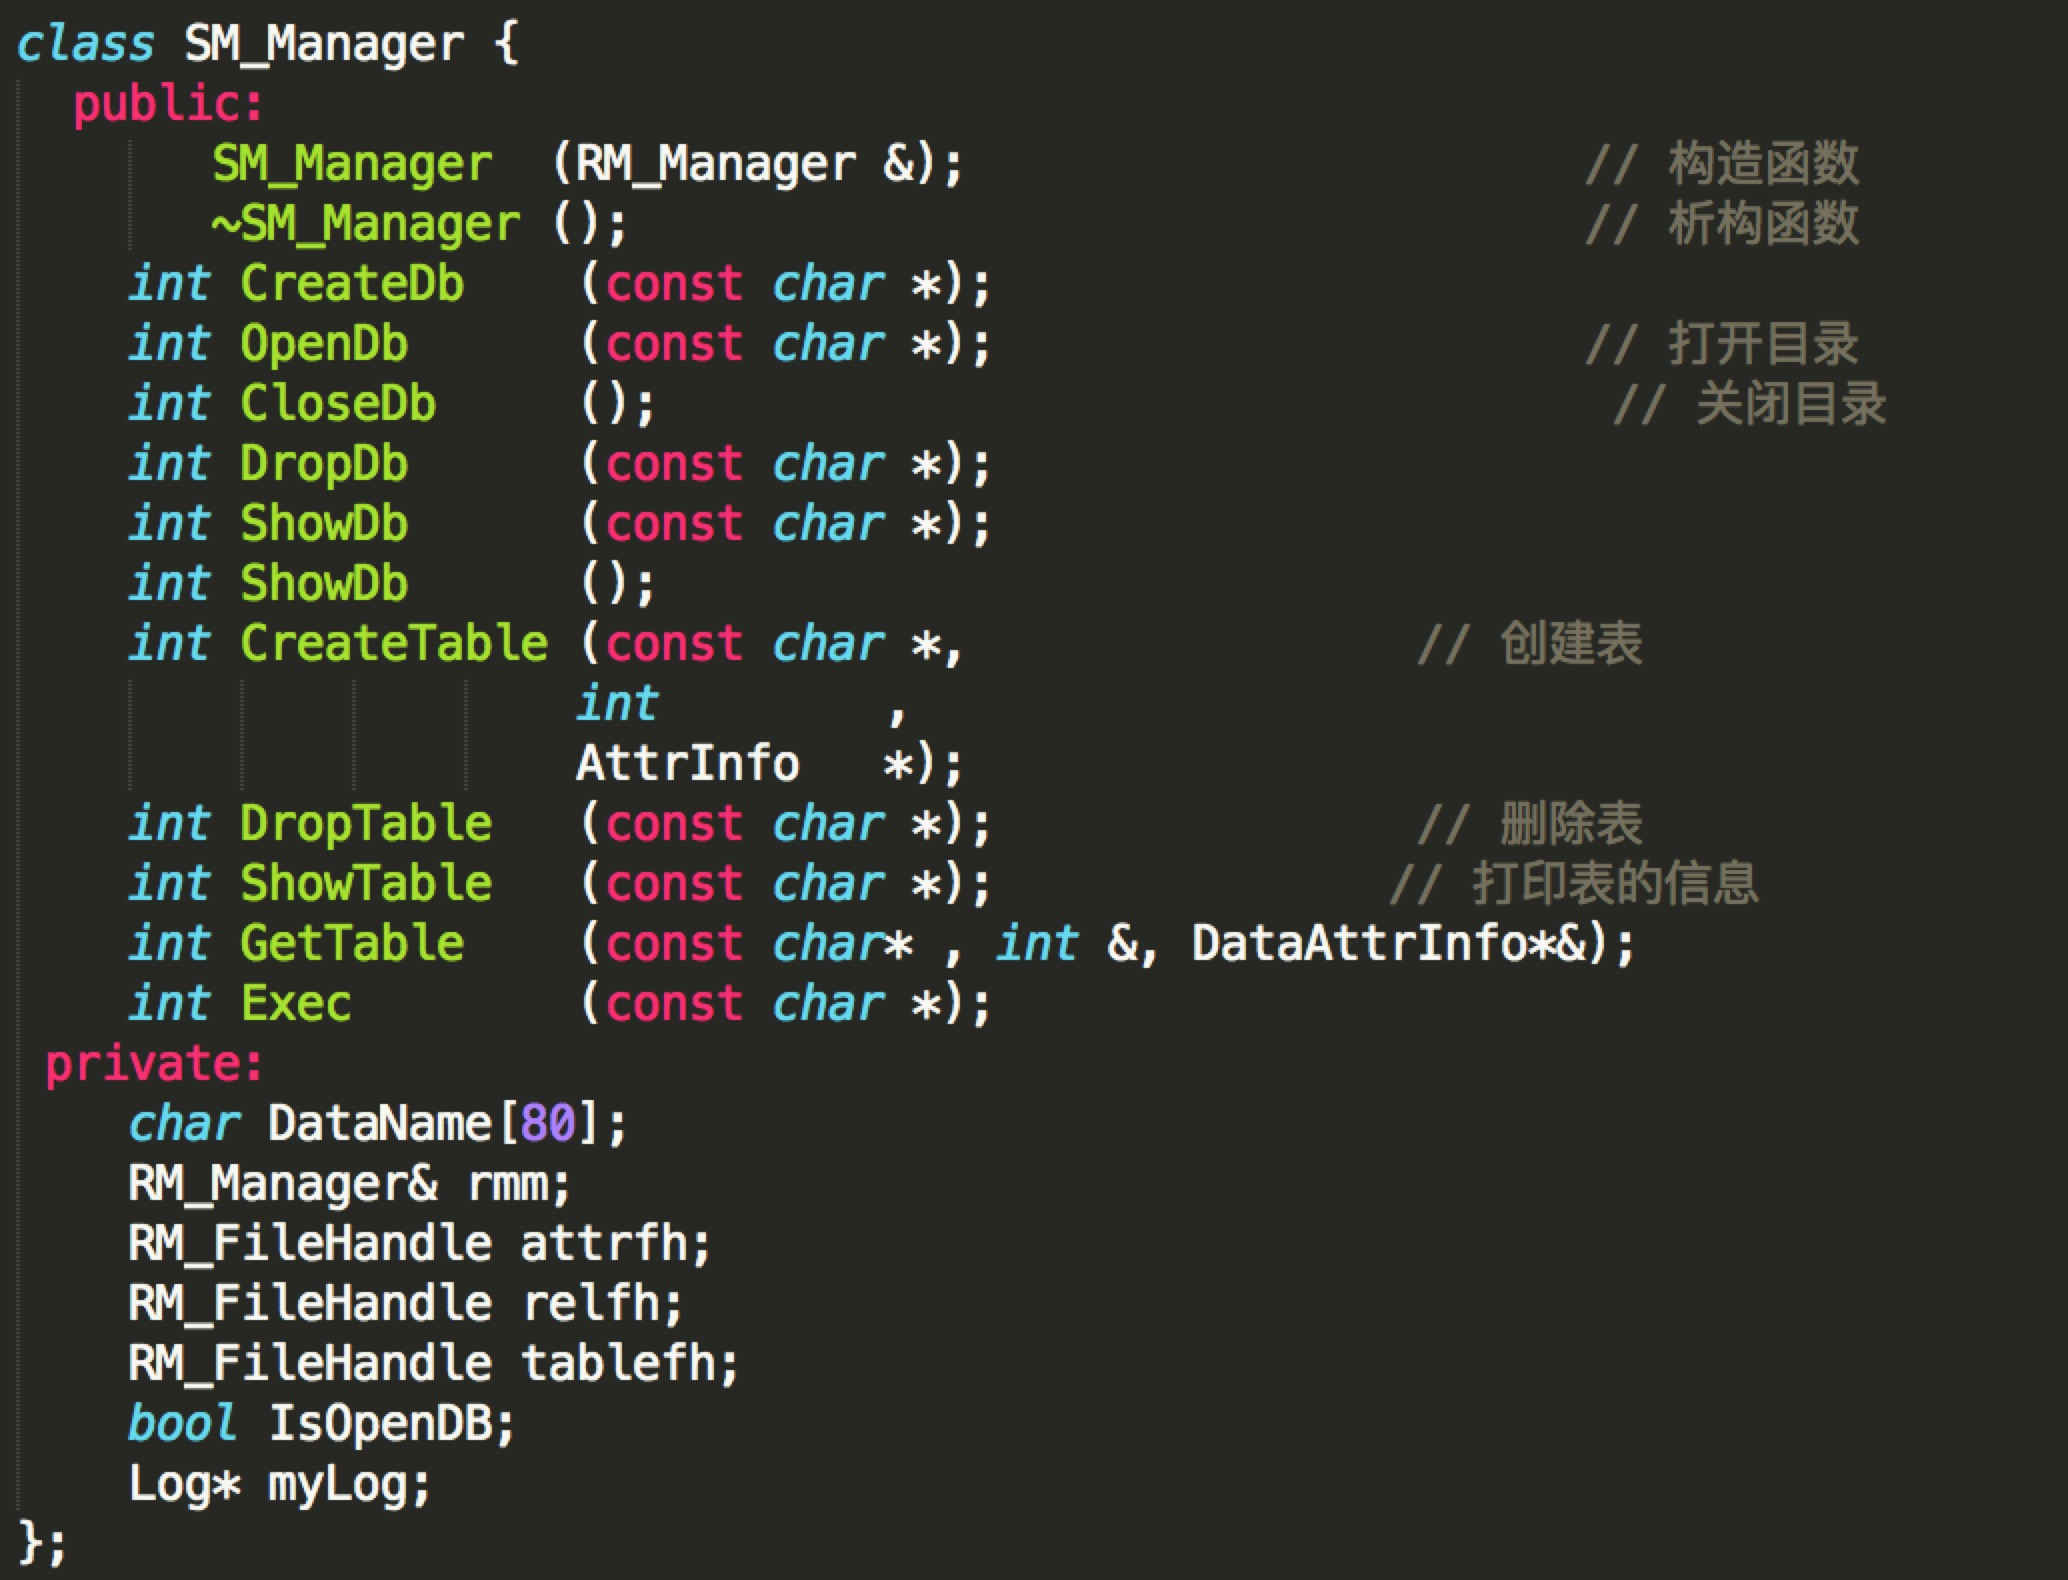
\includegraphics[width=5in]{Figures/SM_Manager.jpg}
\end{figure}

为了实现这几个操作,所采取的方法是在创建数据库的时候首先需要创建一个相关的文件夹,然后在该文件夹下创建两个文件,一个是属性值列表,一个是关系列表。在删除一个数据库时,需要将该文件夹下所有文件全部删除。而新建一个表的时候需要将该表的属性添加到属性表中和数据库表中。而在属性表中每一项包含如下的信息:

\begin{figure}[H]
\centering
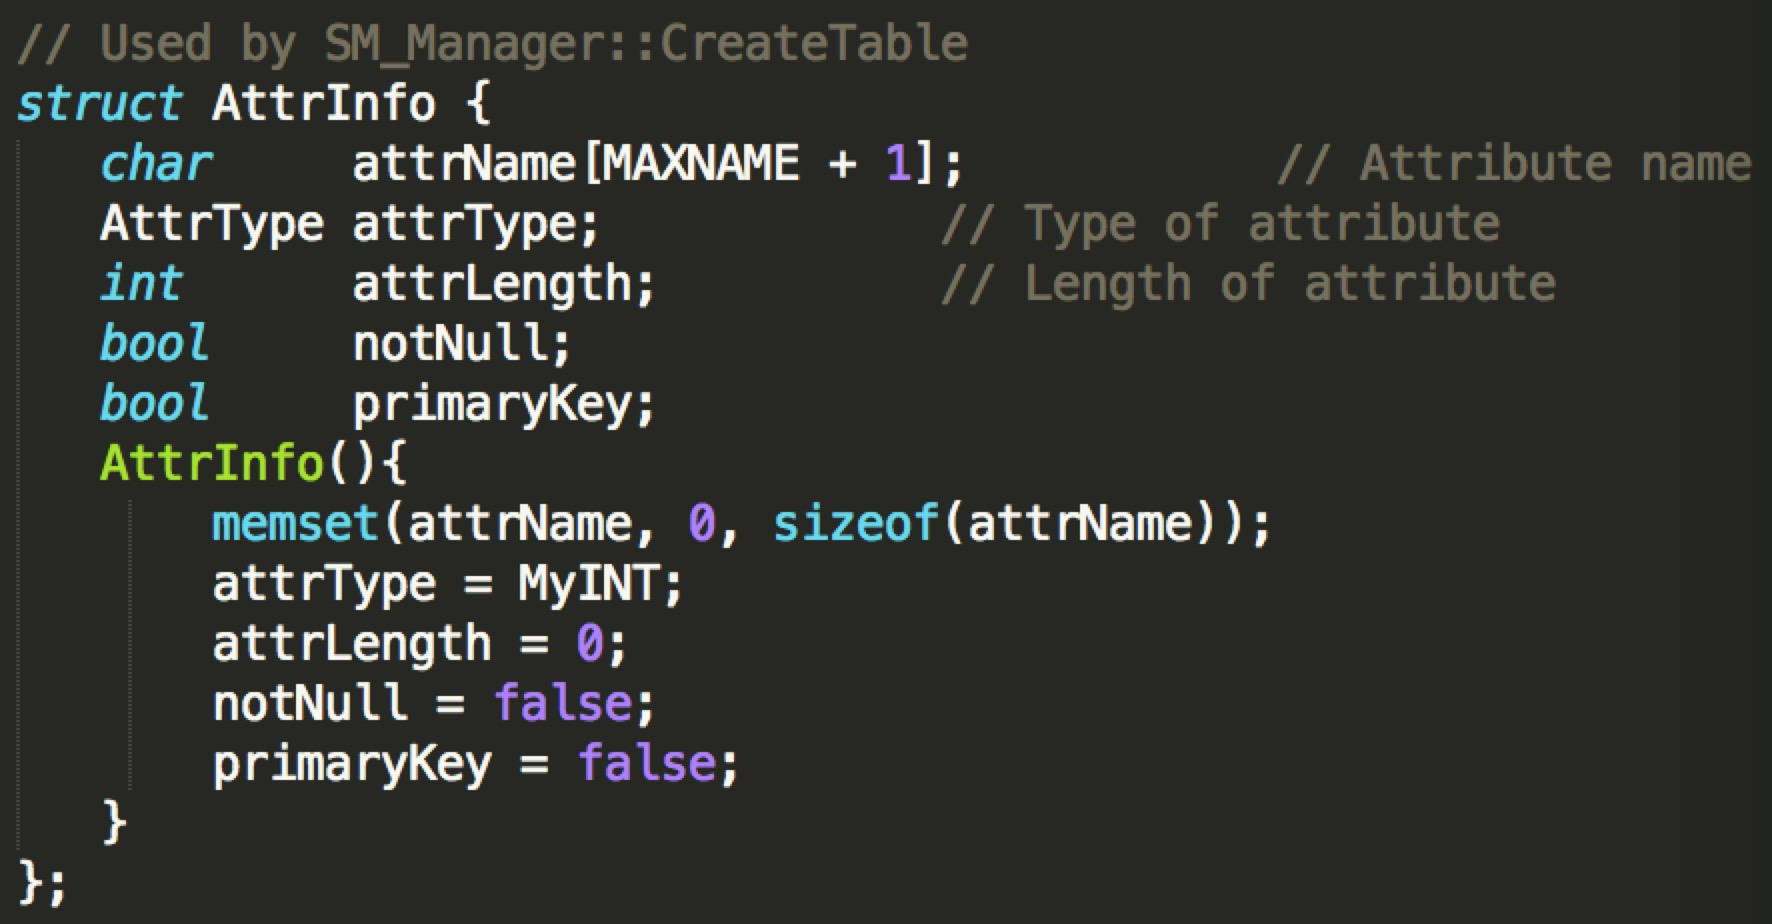
\includegraphics[width=4.2in]{Figures/AttrInfo.jpg}
\end{figure}

在关系列表中需要记录每个用户表的名字。故类的定义如下:
\begin{figure}[H]
\centering
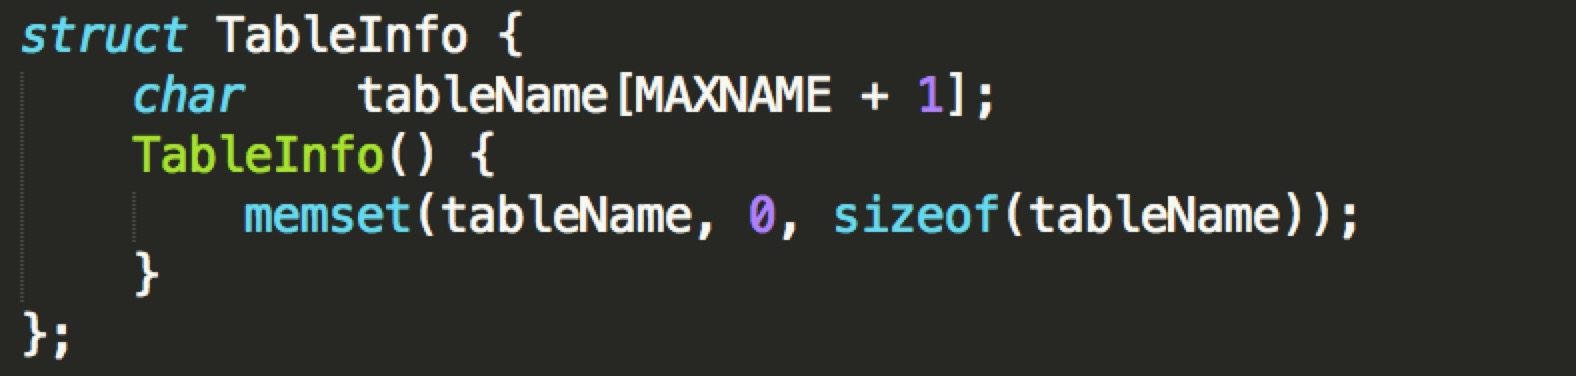
\includegraphics[width=4.2in]{Figures/TableInfo.jpg}
\end{figure}

\section{查询解析模块}

查询模块需要根据指令解析模块Parse\_Manager得到的结果来查询出正确的结果。解析模块传入以下三种参数:

Value类
\begin{figure}[H]
\centering
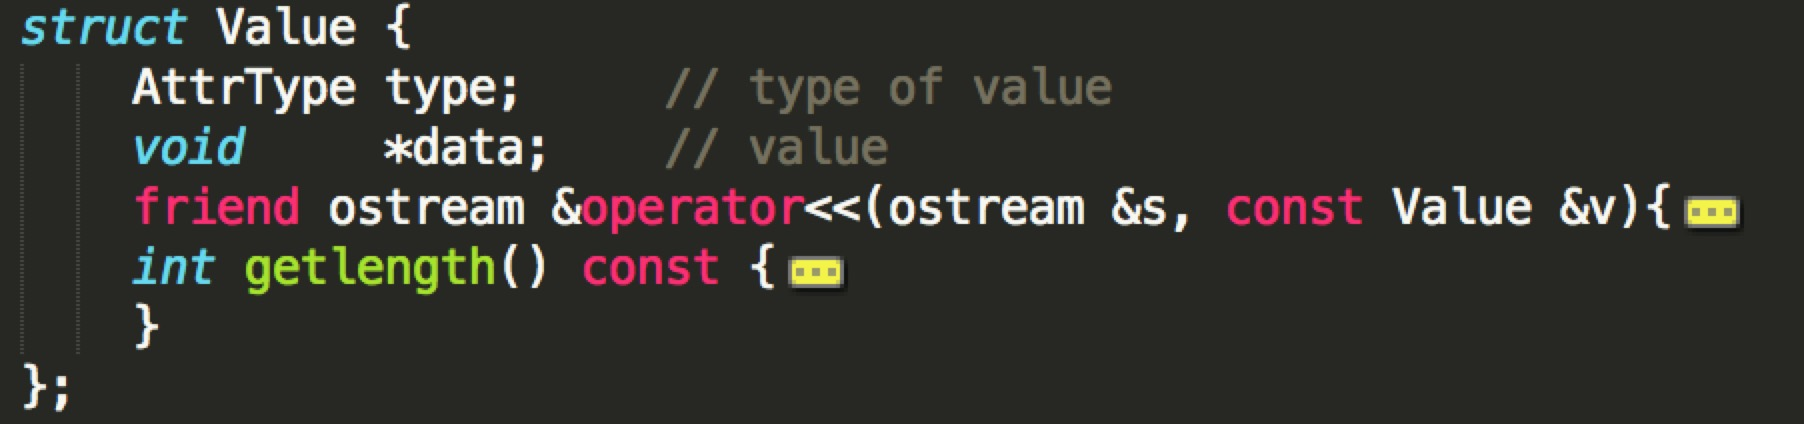
\includegraphics[width=4.2in]{Figures/Value.jpg}
\end{figure}

type为数据类型;Data将数据转化为void*的指针。

condition类
\begin{figure}[H]
\centering
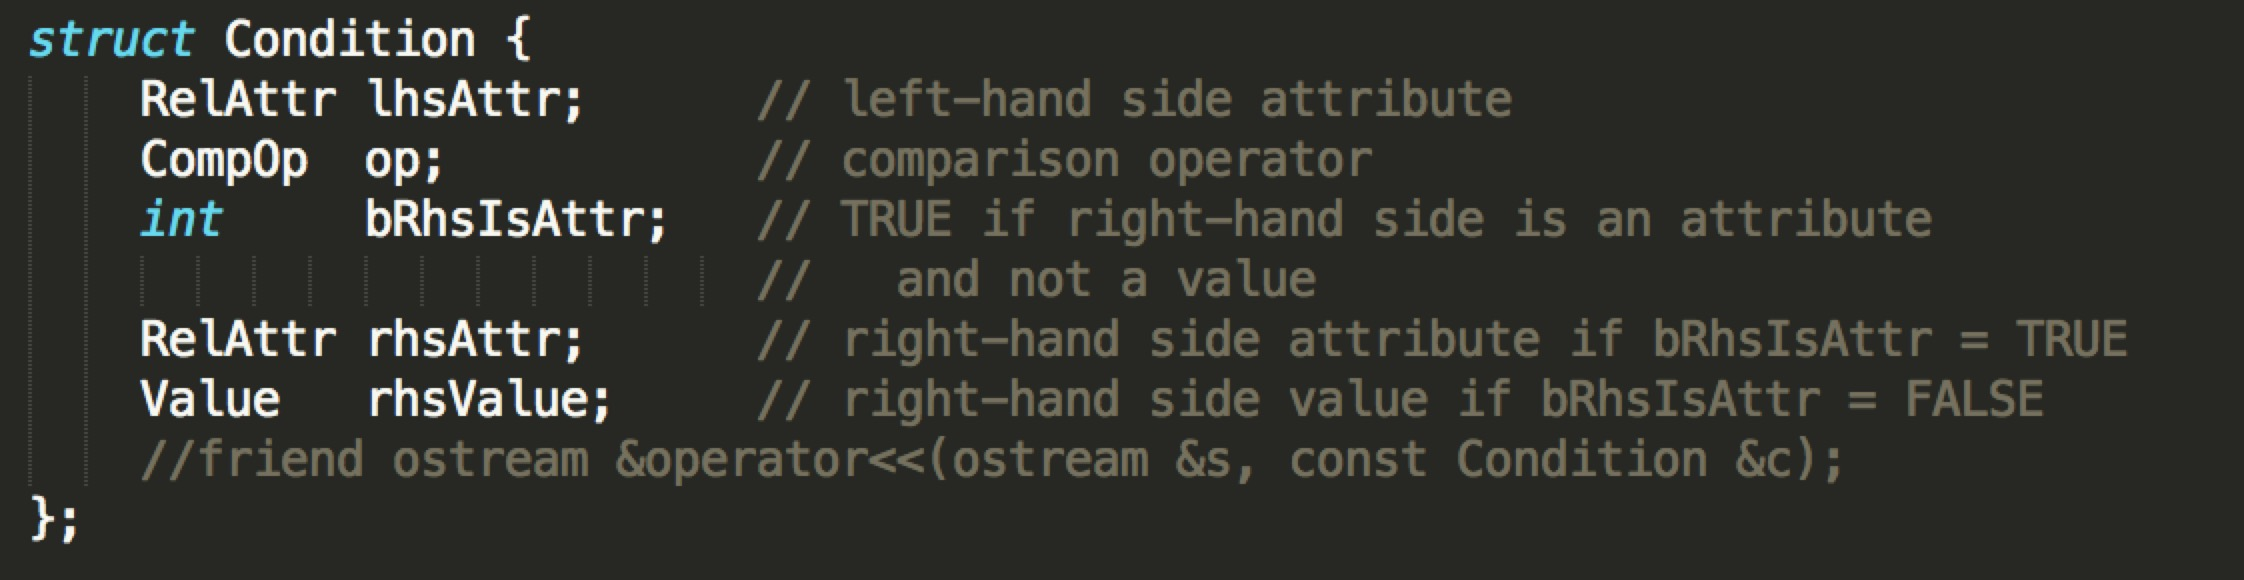
\includegraphics[width=4.2in]{Figures/Condition.jpg}
\end{figure}
lhsAttr为左侧的属性值;op判断符号;bRhsIsAttr为右侧是否为属性值。如果是属性值则rhsAttr为右侧属性值,如果不是则rhsValue为右侧的值

relation类
\begin{figure}[H]
\centering
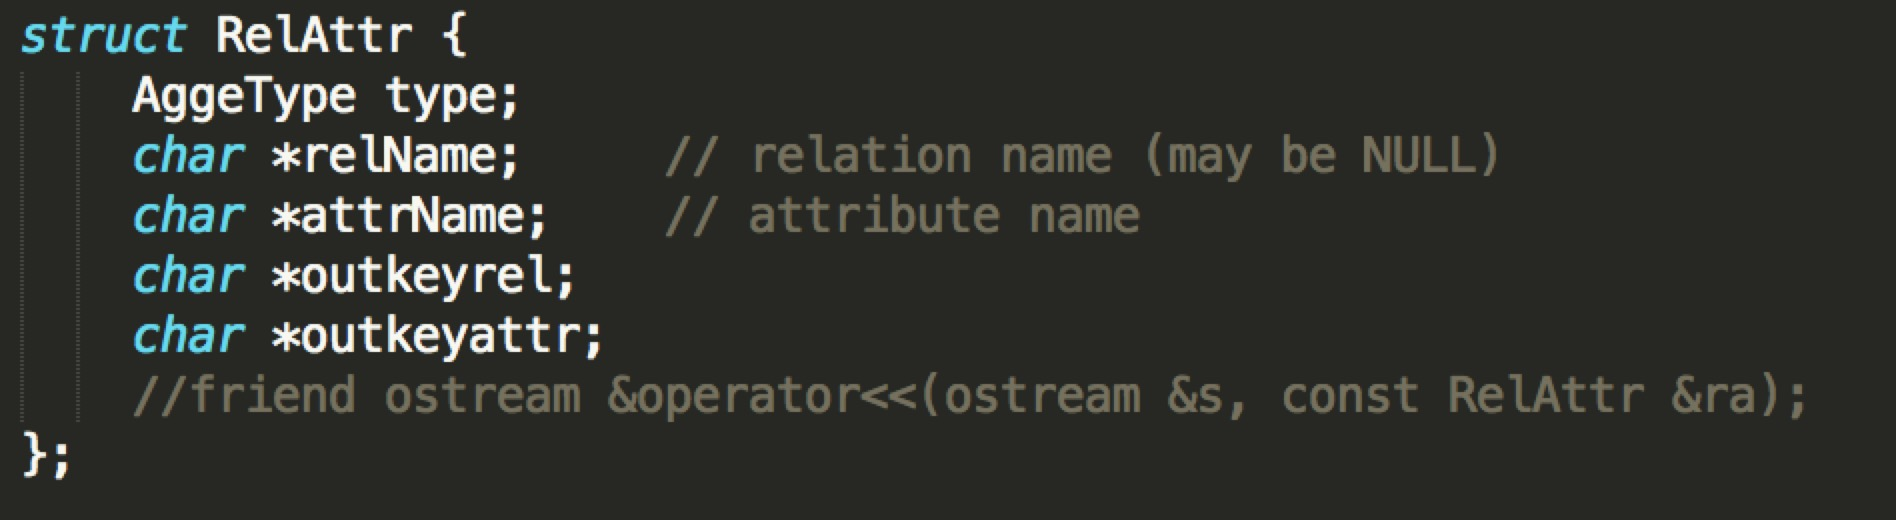
\includegraphics[width=4.2in]{Figures/relAttr.jpg}
\end{figure}

type为数据类型;relName为所属关系名称;attrName为属性名称;outkeyrel为关联关系名称;outkeyattr为关联关系属性


Ql\_manager负责整合前几个模块,其类结构如图所示:
\begin{figure}[H]
\centering
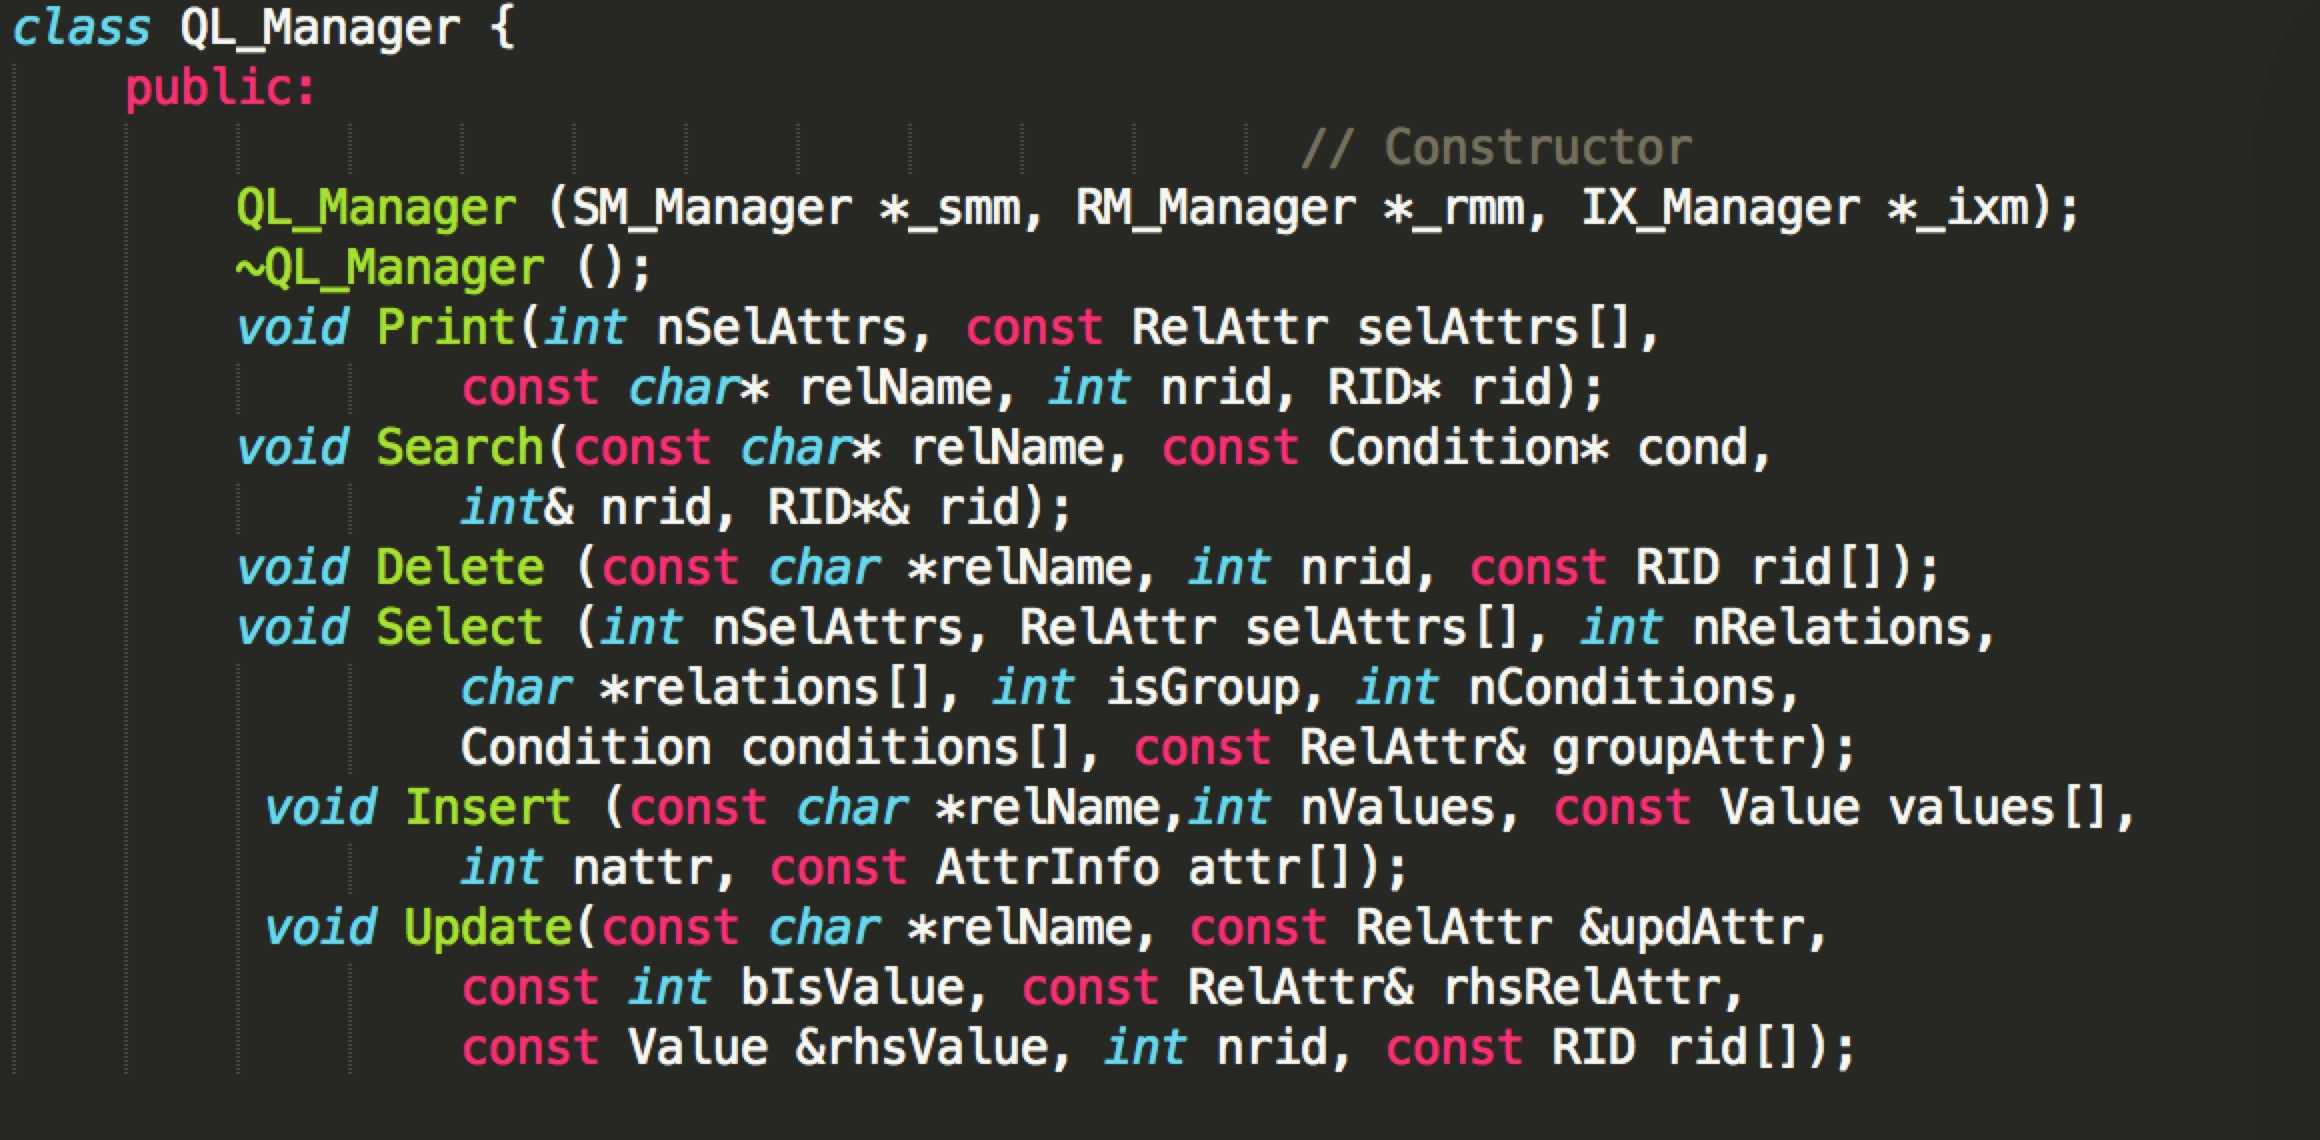
\includegraphics[width=5in]{Figures/QL_Manager.jpg}
\end{figure}

其中五个主要部分说明如下:

(1)void Insert(const char  *relName, int  nValues, const Value values[],int nattr, const AttrInfo attr[])
根据输入的关系名字和value域个数以及各个value的值插入到表中,如果插入时提供了有属性列表,那么需要将其他位置的值置为null,需要注意的是如果该属性为not null,提示本条插入信息无效。

(2)void Print(int nSelAttrs, const RelAttr selAttrs[], const char* relName, int nrid, RID* rid)
根据之前查询所得到的RID列表,某一个Relation中对应的属性依次输出。先判断select域是否为*,如果是,则需要查询attr列表,并且将所有的属性值返回,如果不是,查询attr文件,根据属性名字和关系名字查询出所有需要输出的属性并且依次存放。

(3)void Update(const char *relName, const RelAttr \&updAttr, const int bIsValue, const RelAttr\& rhsRelAttr, const Value \&rhsValue, int nrid, const RID rid[])
更新数据库,将rid列表中所有项依次取出,根据updata的set域中的每一个条件,更新每一个记录。其操作类似于print操作,首先需要查询属性列表,获得相应的每一个属性信息,包括offset等,然后在记录中找到相关属性的位置,然后判断是否为null,然后更新记录,使用filehandle根据Rid来update。

(4)void Delete(const char *relName,int nrid, const RID rid[])
删除rid中的每一项,使用filehandle根据rid来删除记录。

(5)void Search(const char* relName, const Condition* cond, int\& nrid, RID*\& rid)
这一部分是select, print, delete之前的必要操作,该部分的作用是根据条件域得到一个rid列表,这里是一个关系,一个条件下的所有rid列表,rid列表得到后根据交并操作得到最终的rid列表传给以上的三个函数。

(6)void Select (int nSelAttrs, SelAttr selAttrs[], int nRelations, char relations[], int isGroup, int nConditions, Condition conditions[], const RelAttr\& groupAttr) 
这一部分用于处理多表查询以及其他的一些特殊模块。另外还处理一些特殊情况,包括select*,没有from等。这一部分将search和print功能整合起来。对于多表查询部分在3.6.4部分有详细说明。如果在select的时候没有from域,那么求出该表中的所有rid。

最后,在每一个部分中都需要进行相关的判错处理,增加系统的鲁棒性。在任何操作时都要判断relation名字是否在当前数据库中存在,并且需要判断属性值是否也在该数据库中存在,如果存在缺省的关系名称,需要在数据库中搜索该属性值,如果存在两个或者以上关系表具有该属性名称,则需要报错处理。在插入时,当插入数据类型与数据库中该属性不匹配时报错处理,并且根据该属性值是否为Not null判断插入是否合法。相对应的,在更新数据库的时候也需要做类似的判断。

\section{语句解析模块}

语句解析模块负责将SQL语句进行解析,生成相应的关系代数表达式,并调用查询解析模块的函数进行插入、删除、查找等操作。我们采用正则表达式匹配的方法进行语句的解析工作,并对一些语法错误进行了检查。

由于Python语言对正则表达式的处理很好,所以在语句解析模块调用Python来进行正则表达式的匹配,并按照规定的格式将匹配的结果输出到临时文件。在Parse\_Manager中读取临时文件的中间表达形式,并根据语句调用正确的函数。

\begin{figure}[H]
\centering
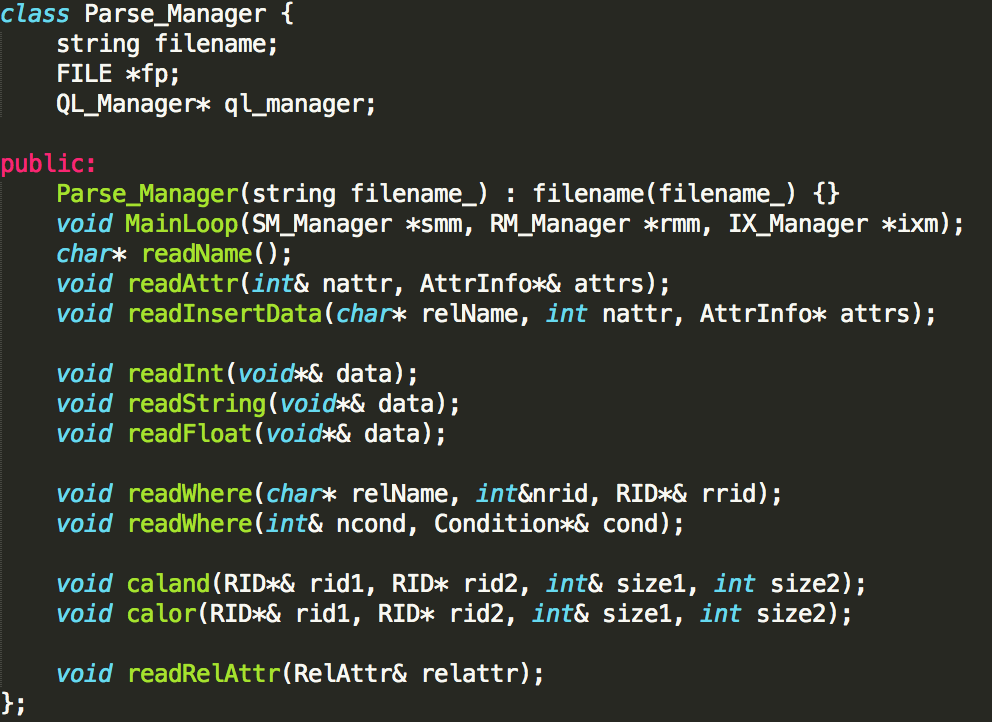
\includegraphics[width=5in]{Figures/Parse_manager.png}
\end{figure}

其中fp为Python解析原始SQL语句后产生的临时文件的句柄。其包含的函数功能为:(1)readAttr:读入属性信息,共nattr个;(2)readInsertData:读入插入数据;(3)readInt:读入一个整数;(4)readFloat:读入一个浮点数;(5)readString:读入字符串;(6)readWhere:读入Where子句;(7)readRelAttr:读入关系表信息。

其中Where子句的读入被重载了两次,第一个为利用栈进行表达式计算,第二个为多表连接等操作时不考虑Where子句含有表达式情况。具体Where表达式计算见附加功能部分。


\section{索引模块}
索引模块的功能是为表中的某一属性建立索引,提高查询速度。

我们项目中索引使用B+树的数据结构实现,每个索引存放在一个独立的文件中。索引文件的命名方式是RelName.AttrName.index。索引文件由页式文件系统管理,有三种页,分别是索引文件头页、中间节点页、叶子节点页。

具体地,索引文件头页按以下方式组织:
\begin{figure}[H]
\centering
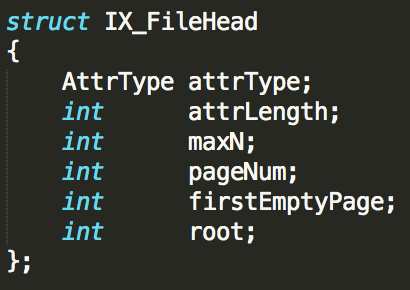
\includegraphics[width=2.5in]{Figures/IX_FileHead.png}
\end{figure}

 索引文件头页中记录索引数据的类型、长度、每页最多放多少索引项、已使用页的数量、根节点页等。

 之后的每个页页头也需要记录一些内容,包括
 \begin{figure}[H]
\centering
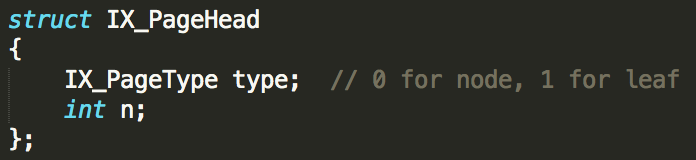
\includegraphics[width=4in]{Figures/IX_PageHead.png}
\end{figure}

type表示该页是中间节点还是叶子节点,n表示该页当前有的索引项个数。

中间节点页与叶子节点页的数据结构是相同的,如下图所示。
\begin{figure}[H]
\centering
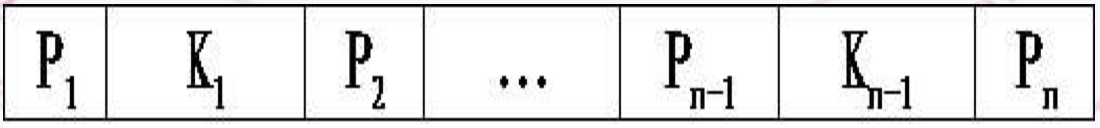
\includegraphics[width=4in]{Figures/indexstruct.png}
\end{figure}

其中P为指针,K为索引码值。区别在于,如果是中间节点,指针指向子节点(索引文件内的一个页),即P存储的是本文件的一个RID;如果是叶子节点,每个索引码值对应一条数据记录,P存储的是该记录在数据表页中的RID;叶子节点最后一个索引码值后面的指针P指向后面一个叶子节点,这样一个索引文件中存储的所有索引项按顺序可以形成一个列表。

索引的插入、删除、查询等功能按照B+树的要求实现。

索引模块的实现仿照记录管理模块,主要包括3个类,即 IX\_Manager、IX\_IndexHandle 以及 IX\_IndexScan。

\begin{figure}[H]
\centering
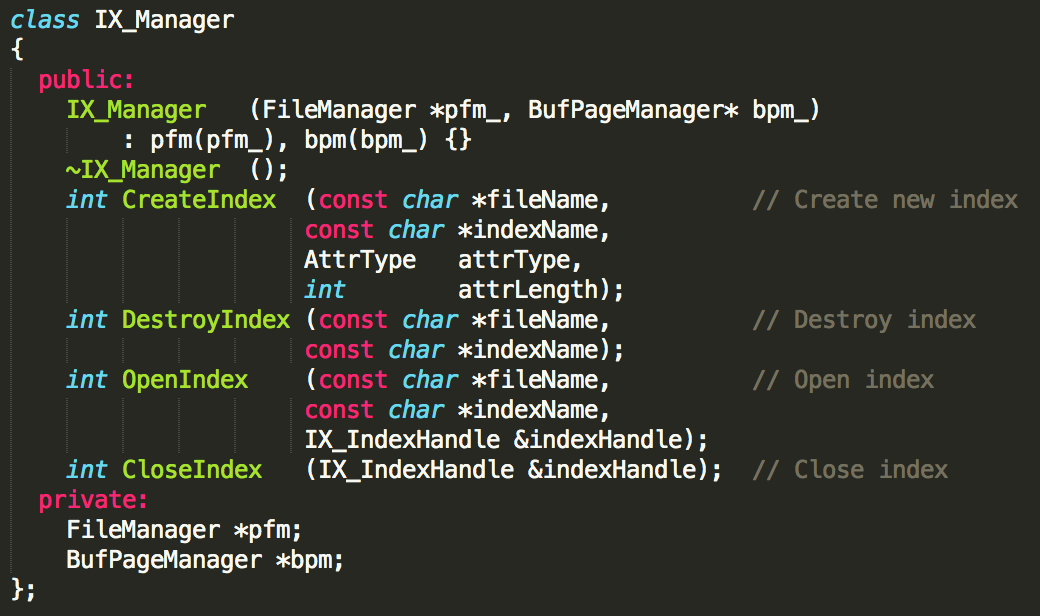
\includegraphics[width=4.5in]{Figures/IX_Manager.png}
\end{figure}

IX\_Manager提供的接口包括新建索引、打开索引、关闭索引和删除索引。

\begin{figure}[H]
\centering
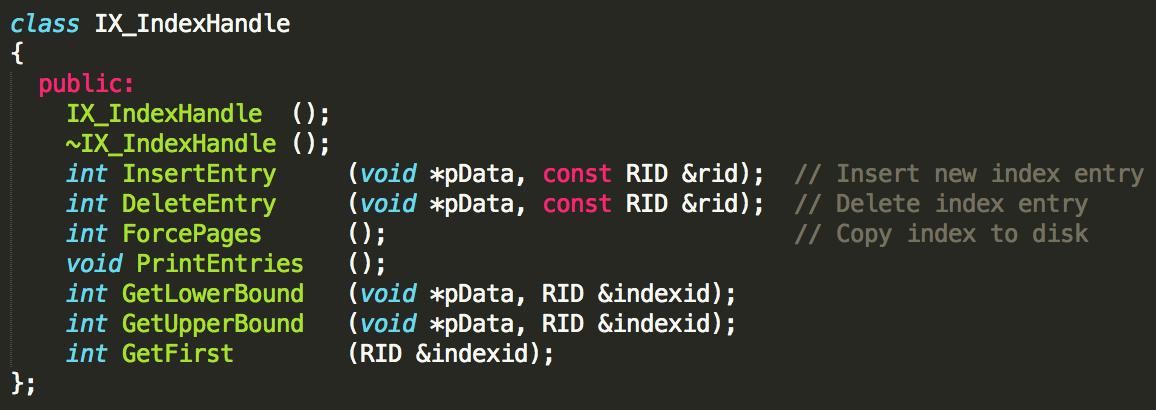
\includegraphics[width=5.5in]{Figures/IX_IndexHandle.png}
\end{figure}

IX\_IndexHandle提供的接口包括插入索引项、删除索引项,以及为了支持查询提供首项、LowerBound和UpperBound的查询。B+树的主要功能实现在这个类中完成。

\begin{figure}[H]
\centering
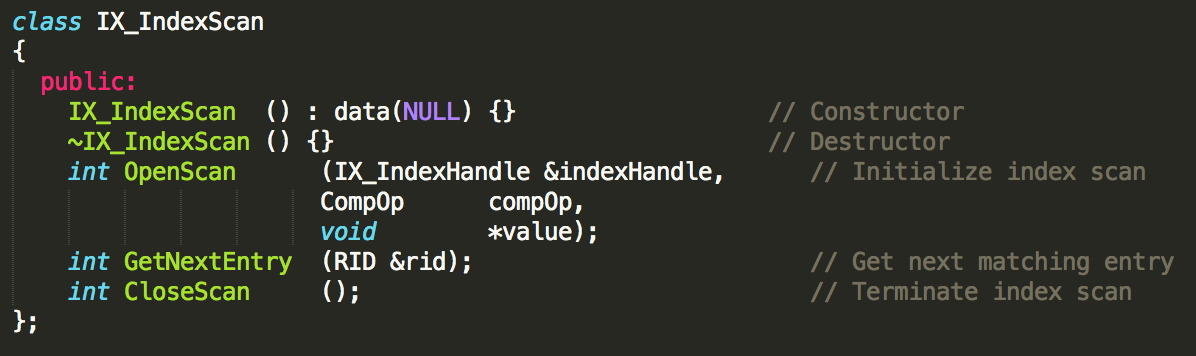
\includegraphics[width=5.5in]{Figures/IX_IndexScan.png}
\end{figure}

IX\_IndexScan提供的接口和RM\_FileScan完全一致,区别在于IX\_IndexScan的查询操作是通过索引在B+树上完成的,效率更高。

其他的模块在执行新建索引以及插入、删除、更新记录的同时,要更新相关的索引。

\section{扩展功能}

\subsection{扩展数据类型}

我们除了整数(int)和字符串(string)外,还扩展了浮点数(float)类型,支持建表时指定float的宽度,即精度。同时在插入数据时可以有float的表达式计算,在查找语句select时可以对float类型查找。由于float基本原理与int一致,故不再赘述。

\subsection{域完整性约束}
域完整性约束,即建表时有CHECK关键字,约束某一个属性可能的取值。

为实现这一功能,我们对每个有域完整性约束的属性,新建一个和索引文件一样的约束文件,命名方式为RelName.AttrName.check.index,也用IX\_Manager管理。在这个文件中,将该属性可能的取值作为索引项依次插入。

插入记录时,检查所有有域完整性约束的属性值是否在其约束文件中存在。如果存在,允许插入,否则拒绝并报错。

\subsection{外键约束}
外键约束,用于与另一张表的关联,以保持数据的一致性。外键一定是另一张表的主键,因此一定是建好索引
的。

所以,在更新一个有外键约束的记录时,打开关联表的主键索引,检查更新后的值是否存在。如果存在,允许更新,否则拒绝并报错。

\subsection{模糊匹配}

模糊匹配支持LIKE关键字以及“\%, *, ?"通配符。其中\%匹配零个或多个字符,* 匹配一个或多个字符,?匹配零个或一个字符。模糊匹配的实现在RM\_FileScan中实现,增加操作符LIKE\_OP表示模糊匹配查询。

在模糊匹配时,考虑到匹配的鲁棒性以及正确性,我们采用了Python正则表达式的方法,这样可以减少错误发生的几率。这时我们仅需要将\%, *, ?换成Python中对应的正则表达式匹配的语法即可。

\begin{figure}[H]
\centering
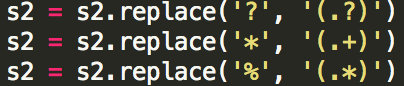
\includegraphics[width=3in]{Figures/vague.png}
\end{figure}

\subsection{复合查询条件}

复合查询条件指WHERE部分可以有更复杂的逻辑表达。

对于Where子句的处理部分,支持Where条件的逻辑表达式形式,即通过逻辑词and,or和括号连接的逻辑表达式。为了实现此功能,我们在Parse\_Manager中得readWhere函数中建立两个栈用于存储操作数(RID的列表)和操作符(包括'and', 'or', '(', ')'),并根据优先级顺序进行计算。每次遇到一个条件,首先通过search函数查找符合此条件的RID的集合,然后通过and,or运算求这些RID集合的交或并。等到所有的条件输入完毕,将求出的RID的集合对应的记录值输出。

\subsection{三个表以上的连接}
三个表以上的查询实现在select函数中,所采取的方式是笛卡尔积的方式,首先读出每一个表中所有的RID,存放在各自的列表中,然后生成一系列的笛卡尔积,然后类似查询解析中select的实现,根据value域对结果进行筛选。

\subsection{聚集查询}
聚集查询根据要求支持4个操作,MAX,MIN,AVG和SUM,分别为最大,最小,平均和总和,这一部分的实现在select函数中实现,根据传入参数中是否具有聚集属性来判断是否需要返回聚集查询结果。该部分实现比较简单,只需要在输出的时候根据聚集属性将结果取最大,最小,平均和求和即可,其中求平均时需要统计一个总数。

\subsection{图形用户界面}
图形用户界面使用Qt实现,在文本框中输入SQL语句,点击后通过命令行执行,然后将输出的结果以表格形式显示。

% Chapter Template

\chapter{实验成果} % Main chapter title

\label{Chapter4}

\section{基础功能}

\ 
% Chapter Template

\chapter{小组分工} % Main chapter title

\label{Chapter5} % Change X to a consecutive number; for referencing this chapter elsewhere, use \ref{ChapterX}


 
% Chapter Template

\chapter{实验总结} % Main chapter title

\label{Chapter6} % Change X to a consecutive number; for referencing this chapter elsewhere, use \ref{ChapterX}



 

%----------------------------------------------------------------------------------------
%	BIBLIOGRAPHY
%----------------------------------------------------------------------------------------

% \printbibliography[heading=bibintoc]

%----------------------------------------------------------------------------------------

\end{document} 